%%%%%%%%%%%%%%%%%%%%%%%%%%%%%%%%%%%%%%%%%%%%%%%%%%%%
\graphicspath{{}{introduction/}{Diagrams/}}

\section{The Standard Model}

The Standard Model (SM) of particle physics is a Yang-Mills theory~\cite{Yang:1954ek} of strong, weak and electromagnetic (EM) particle interactions based on an $SU(3) \times SU(2) \times U(1)$ local gauge symmetry. The first remarkable aspect of the theory is in the fact that it relies on the same idea that explains Maxwell's equations, the principle of gauge invariance. In this way, it is hard to pin down the official conception of the SM, although widely associated with the works of Sheldon L. Glashow~\cite{Glashow:1961tr}, Steven Weinberg~\cite{Weinberg:1967tq} and Abdus Salam~\cite{Salam:1968rm}. Unconcerned with quarks and the strong force, they proposed a spontaneously broken $SU(2) \times U(1)$ local gauge symmetry for leptons, which already reflected most of what we know about the electroweak (EW) interactions nowadays. In fact, the spontaneous broken symmetry that was used already predicted the existence of a charged massive vector boson, the $W^\pm$, a neutral massive vector boson, the $Z$, and of a massless generator of the unbroken $U(1)_{\rm EM}$ group, the photon $\gamma$. Beyond unifying the weak and EM forces, the breaking through the Higgs mechanism~\cite{Higgs:1964ia,Higgs:1964pj} implied that an additional scalar particle, the Higgs boson $H$, had to exist. This last prediction was experimentally validated after the discovery of a neutral scalar boson at the LHC in 2012~\cite{Chatrchyan:2012xdj,Aad:2012tfa}, the last SM particle to be experimentally observed.

The strong force had a much richer and more turbulent history. The quark model, developed by Murray Gell-Mann and George Zweig~\cite{Zweig:1981pd,GellMann:1964nj} in 1964, had great success in explaining the growing number of hadronic resonances found by experiments. However, it was not until asymptotic freedom was discovered in non-Abelian gauge theories~\cite{Gross:1973id,Politzer:1973fx} that quantum chromodynamics (QCD) was really born. QCD is an $SU(3)$ local gauge theory describing the interaction of quarks and gluons, and is vastly different from any other theory we will encounter in this thesis. Its uniqueness is best exemplified through color confinement, the property that colored particles must always be present in bound colorless states, called hadrons. For QCD, confinement is guaranteed below the scale $\Lambda_{\rm QCD} \approx 250$ MeV, below which strong processes are non-perturbative. This is to be contrasted with asymptotic freedom, where the strong interactions between quarks and gluons become asymptotically weaker at higher energies. The presence of new degrees of freedom other than quarks and gluons at low energies, namely the hadrons, is a clear evidence of a phase transition and makes QCD a unique topic within the SM. At times we will refer to known results in this theory, but it usually has little bearings on electroweak physics.

\subsection{Fields and symmetries}

We now set out for a more precise definition of the SM field content, discussing some details of local gauge invariance. All fermion fields in the SM are Weyl fields of either definite left-handed (LH) or right-handed (RH) chirality. An equivalent statement is that SM fields are eigenvectors of $\gamma_5$: $\gamma_5 \psi_R = \psi_R$ for RH, and $\gamma_5 \psi_L = - \psi_L$ for LH fields. This is an important feature that allows us to work with 2 component Weyl spinors and makes explicitly manifest the chiral nature of weak interactions. The LH field content and their representation under the different gauge groups is shown in \reftab{tab:SMcharges}. Note that only LH particles transform non-trivially under $SU(2)_L$. Also shown is the Higgs field $H$, a complex scalar field, doublet under $SU(2)$. As we will see in the next section, $H$ is responsible for the breaking of $SU(2)_L \times U(1)_Y \to U(1)_{\rm EM}$.
%
\renewcommand{\arraystretch}{1.4}%
\begin{table}[t]
 \begin{tabular}{lccccccccccc}
 \hline
    & $Q_L^\alpha$& $L^\alpha$ & $\overline{u_R^\alpha\vphantom{d}}$ & $\overline{d_R^\alpha}$ & $\overline{e_R^\alpha\vphantom{d}}$ & &$H$ & & $G$ & $W$ & $B$\\
    \hline
  SU$(3)_c$ & $\bm{3}$ & $\bm{1}$& $\overline{\bm{3}}$ & $\overline{\bm{3}}$ & $\bm{1}$ & & $\bm{1}$ & & $\bm{8}$ & $\bm{1}$ & $\bm{1}$ \\
  SU$(2)_L$& $\bm{2}$ & $\bm{2}$ & $\bm{1}$ & $\bm{1}$& $\bm{1}$& & $\bm{2}$ & & $\bm{1}$ & $\bm{3}$ & $\bm{1}$ \\
  U$(1)_Y$ & $1/3$ & $-1$ & $-4/3$ & $2/3$ & $2$ & & $1$ & & $0$ & $0$ & $1$ \\
  \hline
 \end{tabular}
 \caption[SM field content.]{The representation of the left-handed Weyl fields, the complex scalar and gauge bosons under each gauge group of the SM. For $U(1)_Y$, the charge is shown instead. All fermions carry a flavour index $\alpha = e, \mu$ or $\tau$.\label{tab:SMcharges}}
\end{table}
\renewcommand{\arraystretch}{1.0}%
%
From the observed EM charges $Q_{\rm EM}$, the $SU(2)_L$ isospin $T_3$, and by virtue of the Gell-Mann-Nishijima formula~\cite{Nakano:1953zz,Gell-Mann:1956iqa}
%
\begin{equation}
 Q_{\rm EM} = T_3 + \frac{Y}{2},
\end{equation}
%
the hypercharge $Y$ of each SM field is fixed. The \emph{local} gauge transformation of the matter fields are given by
\begin{equation}
\psi  \to \exp{i g \theta^a(x) T^a } \psi,
\end{equation}
where $g$ is the gauge coupling constant, $a$ counts the number of generators $T^a$, and $\theta^a(x)$ are arbitrary parameters that depend on space-time coordinates $x^\mu$. To achieve local gauge invariance, we require the following gauge fields associated with each group:
%
\begin{equation}
 SU(3)_C: \{G_1 (x), \cdots, G_8 (x)\}, \quad SU(2)_L:  \{W_1(x), W_2(x), W_3(x)\}, \quad U(1)_Y: B(x),
\end{equation}
%
corresponding to the eight gluons, the $SU(2)$ gauge fields and the hypercharge field. Note that the number of gauge fields matches the number of generators in each group, \eg\ for $SU(N)$ there are $N^2 -1$ generators. For the original $SU(2)\times U(1)$ theory, this implied that in addition to the charged gauge fields, which explained Fermi's theory for beta decays, and the observed massless photon, there must have been an additional neutral gauge field corresponding to some linear combination of $W^3$ of $SU(2)_L$ and $B$ of $U(1)_Y$. This striking prediction was in fact first confirmed by Gargamelle through the observation of accelerator neutrinos scattering into final states with no charged leptons~\cite{Hasert:1973ff}. 

The generators of a given symmetry group equipped with commutators form a Lie Algebra, obeying $[T^a, T^b] = i f^{abc} T_c$, with $f^{abc}$ being the group structure constant. In the special case $f^{abc} = 0$, the generators commute and the group is said to be Abelian, like in the case of $U(1)_Y$. Otherwise, the group is non-Abelian and the theory displays a much richer underlying dynamics. The SM is a non-Abelian theory, since its symmetry group contains direct products of two $SU(N)$ groups with $N > 1$. We now illustrate how to build a gauge-invariant Yang-Mills Lagrangian, like that of the SM. Take an $a$-dimensional Yang-Mills theory and define $\bm{\theta} = T^a \theta^a$ and $U = e^{i g \bm{\theta}}$. We can now perform gauge transformations on the relevant matter fields $\psi$, gauge fields $\bm{A}_\mu = T_a A_\mu(x)^a$ and derivatives of matter fields as follows
%
\begin{equation}
\psi \to U \psi, \quad \bm{A}_\mu \to U \bm{A}_\mu U^{-1} - \frac{i}{g} (\partial_\mu U) U^{-1}, \quad \partial_\mu \psi \to U \partial_\mu \psi +  \psi (\partial_\mu U).
\end{equation}
%
As we can see, the last term is not invariant due to the local character of the gauge transformations. To preserve gauge invariance, a covariant derivative, transforming as $D_\mu \to U D_\mu U^{-1}$, now replaces the ordinary derivative. It is defined as 
\begin{equation}
D_\mu = \partial_\mu + ig \bm{A},\quad \text{such that} \quad D_\mu\psi \to U D_\mu\psi, \,\,\implies\,\,\overline{\psi} i\slashed{D}\psi \to \overline{\psi} i \slashed{D} \psi. 
\end{equation}
%
The invariant term above is the fermion kinetic term. Beyond fermion propagation, it is the main way to describe fermion-gauge interactions in the SM. In particular, the full covariant derivative in the SM is given by
%
\begin{equation}
 D_\mu = \partial_\mu + ig \,W_\mu^a\tau_a + i\frac{Y}{2} g^\prime \,B_\mu + i\frac{g_s}{2} \,G_\mu^b\lambda_b,
\end{equation}
%
where $\tau_a = \sigma_a/2$ are the generators built from Pauli matrices acting on the doublets of $SU(2)_L$, and $\lambda_b$ the generators built from the Gell-Mann matrices acting on the triplet representations of $SU(3)_c$. This also fixes the notation for the gauge couplings in the SM. Finally, the gauge invariant kinetic terms for the gauge bosons are 
%
\begin{equation}
\mathscr{L}_{\rm gauge} = -\frac{1}{4} G^{a}_{\mu\nu} G_a^{\mu\nu} - \frac{1}{4} W^{a}_{\mu\nu} W_a^{\mu\nu} -\frac{1}{4} B_{\mu\nu} B^{\mu\nu},
\end{equation}
%
where $F^a_{\mu \nu} = \partial_\mu F^a_\nu - \partial_\nu F^a_{\mu} - g_F f^{abc} F_{b\,\mu} F_{c\,\nu}$ with $g_F$ the relevant gauge coupling. The kinetic term in Abelian theories concern only the propagation of gauge bosons, however, for non-Abelian groups the term proportional to $g_F$ in $F^a_{\mu \nu}$ introduces interactions among the gauge bosons proportional to $g$ and $g^2$. Therefore, a non-Abelian theory is already an interacting theory without the addition of any matter fields.

\subsection{Spontaneous symmetry breaking}

So far we have only discussed the gauge and fermionic content of the SM. The scalar sector is, in fact, quite special. The only scalar particle, the Higgs boson, is responsible for spontaneously breaking $SU(2)_L\times U(1)_Y$ to $U(1)_{\rm EM}$ after it acquires a non-zero vacuum expectation value (vev). This introduces a mass scale in the theory which, apart from dimensionless couplings, sets the scale of EW physics. Note that because it is a scalar particle, a non-zero vev does not violate the symmetries of space-time, namely Lorentz invariance. The Higgs is a complex scalar field and a doublet under  $SU(2)_L$, and so we can write
%
\begin{equation}
  H =  \frac{1}{\sqrt{2}} \left( \begin{matrix}  G_1^+ + i G_2^+ \\  h^0 + i G_3^0 \end{matrix} \right) =  \frac{e^{i G_a \tau^a}}{\sqrt{2}} \left( \begin{matrix} 0 \\  h \end{matrix} \right).
\end{equation}
%
The Higgs Lagrangian reads
%
\begin{equation}
\mathscr{L}_{\rm Higgs} \supset \left( D^\mu H \right)^\dagger \left( D_\mu H \right) - V(H), \quad {\rm with} \quad V(H) = \mu^2 H^\dagger H + \lambda \left( H^\dagger H \right)^2,	
\end{equation}
%
where $\mu^2$ has mass dimension 2, being the only dimensionful parameter in the SM. If $\mu^2 < 0$, minimizing the potential $V(H)$ requires $\bra{0} H \ket{0} = \left( 0, \,\, v/\sqrt{2} \right)^T$, where $v^2 = - \mu^2 /\lambda$ is the vev chosen to lie in the real and neutral direction. We now can then expand around the true vacuum of the theory by redefining the fields $G_a \to G_a/v$ and $h \to h + v$. At this point, a rewriting of the potential reveals the mass and interactions of every component of the scalar doublet. Note, however, that it contains no mass terms for $G_1$, $G_2$ and $G_3$. These are the Nambu-Goldstone bosons of the theory, and although they are massless, they do possess interactions with the scalar and gauge boson fields. One way to understand their role is to perform an $SU(2)_L \times U(1)_Y$ gauge transformation in our Lagrangian such that the resulting Higgs doublet reads
%
\begin{equation}
H \to e^{- i G_a \tau^a/v} H =  \frac{1}{\sqrt{2}}\left( \begin{matrix}  0 \\ h + v \end{matrix} \right).
\end{equation}
%
This transformation must also be applied to the gauge fields, fixing the gauge. This particular choice is rather convenient and is known as the unitary gauge. We then find
%
\begin{align}
 \mathscr{L}_{\rm Higgs} &\supset - \frac{1}{2} m_h^2 h^2 - \lambda v h^3 - \frac{\lambda}{4} h^4  \nonumber\\ &\qquad\qquad +  M_\textsc{w}^2 W_\mu^\dagger W^\mu \left[ 1 + \frac{2 h}{v} + \frac{h^2}{v^2}\right] + \frac{M_\textsc{z}^2}{2} Z_\mu Z^\mu \left[ 1 + \frac{2 h}{v} + \frac{h^2}{v^2}\right],
\end{align}
%
where $m_h = \sqrt{2\lambda}\, v = 125.18 \pm 0.16$ GeV~\cite{PDG}. Most importantly, after SSB, the Higgs kinetic term has given us three massive and one massless vector bosons, defined as
\begin{equation}
 W^\pm_\mu = \frac{1}{\sqrt{2}} \left(W^1_{\mu} \mp i W^2_{\mu} \right), \quad Z_\mu = c_\textsc{w} W^3_\mu - s_\textsc{w} B_\mu, \quad A_\mu = c_\textsc{w} B_\mu - s_\textsc{w} W^3_\mu.
\end{equation}
% 
where $s_\textsc{w}$ ($c_\textsc{w}$) is the sine (cosine) of the weak angle, defined by $c_\textsc{w} = g/\sqrt{g^2 + g^{\prime\,2}}$. These fields correspond to the mediators of the weak charged-current (CC) interactions ($M_\textsc{W} = g v/2 = 80.387\pm 0.016$ GeV~\cite{PDG}), of the weak neutral-current (NC) interactions ($M_\textsc{z} = M_\textsc{w}/c_\textsc{w} = 91.1876\pm0.0021$ GeV~\cite{ALEPH:2005ab}) and the massless photon $A_\mu$, mediator of the unbroken EM interactions. Their interactions with the Higgs boson are also shown in the triple and quadruple vertex terms above. The interactions with matter are obtained from the fermion kinetic terms, where the charged, neutral and electromagnetic currents are defined and written as
%
\begin{equation*}
\mathscr{L}_{\rm NC} = e \,{J}_\mu^\gamma A^\mu + \frac{g}{c_\textsc{w}}\, {J}_\mu^Z Z^\mu, \quad {J}_\mu^\gamma =  \overline{\psi} Q_{\rm EM} \gamma_\mu \psi, \quad %
{J}_\mu^Z = \overline{\psi} \gamma_\mu \left[ \left( \frac{T_3}{2} - Q_{\rm EM} s_\textsc{w}^2 \right) - \frac{T_3}{2} \gamma^5\right] \psi,
\end{equation*}
\begin{equation}
\mathscr{L}_{\rm CC} = \frac{g}{\sqrt{2}}  \, \left( {J}_\mu^+ W^{\mu \,+} + {J}_\mu^- W^{\mu \,-} \right), \quad
%
{J}_\mu^+ = \frac{1}{2} \overline{\psi}_u \gamma_\mu \left( 1 - \gamma^5\right) \psi_d + {\rm h.c.},
\end{equation}
%
where $\psi \in \{ \nu_L, e_L, u_L, d_L, e_R, u_R, d_R \}$, and $\psi_{u,\,d}$ denoting fermions with $T_3 = \pm 1/2$. From the weak currents we note two important aspects: \emph{i)} weak interactions indeed violate parity with a $V-A$ structure, \emph{ii)} charged-current interactions are purely LH as they should be since no RH fields are charged under $SU(2)_L$. After SSB, only the EM current is conserved $\partial^\mu J_\mu^\gamma = 0$. 

In the discussion above, we fixed the gauge of the SM to simplify the EW Lagrangian. This is not necessary and, in fact, another possibility is to keep all terms involving the Nambu-Goldstone fields $G_a$ and eliminate off-diagonal kinetic terms of the type $Z_\mu\partial^\mu G_3$ by introducing the following gauge breaking Lagrangian to the SM
\begin{equation}
 \mathscr{L}_{\rm R_\xi} = -\frac{\left(\partial_\mu A^\mu\right)^2}{2 \xi_\gamma} - \frac{\left(\partial_\mu Z^\mu + \xi_Z M_Z G_3^0 \right)^2}{2 \xi_Z} - \frac{\left|\partial_\mu W^{\mu\,-} + i \xi_W M_W G^- \right|^2}{2 \xi_W}.
\end{equation}
This is known as the $R_\xi$ gauge, where the explicit dependence on the gauge breaking parameters $\xi$ serves as a useful diagnostic of gauge invariance in physical observables. The Lorentz gauge is recovered for $\xi = 0$ and the Feynman-'t Hooft gauge with $\xi = 1$. This method to fix the gauge played an important role in the development of the SM. First introduced by Ludvig Fadeev and Victor Popov~\cite{Faddeev:1967fc}, this provided a recipe to perform calculations in gauge theories without the ambiguity of the gauge symmetry. In practice, one must also add unphysical ghost fields to guarantee the unitarity of the theory. These only appear in loop processes and we will not encounter them again in this thesis. An additional advantage of fixing the gauge in this way is that it allows us to trace the Nambu-Goldstone degrees of freedom. The pseudo-scalar fields $G^\pm$ and $G_3$ end up behaving very similarly to the $W^\pm$ and $Z$ gauge bosons. In fact, at high-energies it can be shown that the Nambu-Goldstone bosons are equivalent to the longitudinal polarization states of their respective gauge bosons~~\cite{Cornwall:1974km,LlewellynSmith:1973yud}. This is known as the Nambu-Goldstone boson equivalence theorem, and it turns out to be very important to understand processes like $W_L \, W_L$ and $Z_L \,Z_L$ scattering. At very high-energies and without the Higgs boson, such processes grow indefinitely ($\sigma \propto s$), spoiling the unitarity of the $S$-matrix. The fact that this problem was solved by including contributions from $h$ exchange provided a no-lose theorem for the LHC: either the Higgs boson would be discovered, or new physics must appear to unitarize these processes. 

\subsection{Fermion masses}

The EW sector is also responsible for the generation of fermion masses in the SM. As noted before, all LH fermions in the SM are $SU(2)_L$ doublets, just like the Higgs. This allows us to construct the so-called Yukawa terms,
%
\begin{equation}
 \mathscr{L}_{\rm Yukawa}=  y^e_{\alpha\,\beta}  \left(\overline{L}^\alpha H\right) e_R^\beta +  y^u_{\alpha\,\beta}  \left(\overline{Q}^\alpha_L \tilde{H} \right) u_R^\beta + y^d_{\alpha\,\beta}  \left(\overline{Q}_L^\alpha H \right) d_R^\beta  + \,\, {\rm h.c.},
\end{equation}
%
where we defined the charge-parity (CP) conjugated Higgs field $\tilde{H} = i \sigma_2 H^* = ( h^0 + i G_3^0, \,\, G_1^- - i G_2^-  )^T$ and included all three families of fermions by promoting $y^\psi \to \textbf{Y}^\psi$ to a $3\times3$ matrix. . After SSB, these interaction terms endow charged-leptons and quarks with a dirac mass term of the form
\begin{equation}
 m_\psi \overline{\psi} \psi = m_\psi \left( \overline{\psi}_L \psi_R +\overline{\psi}_R \psi_L \right),\quad {\rm with} \quad m_\psi = \frac{y_\psi \, v}{\sqrt{2}},
\end{equation}
where $\psi_{L,\,R} = P_{L,\, R} \, \psi = (1 \mp \gamma_5)\, \psi/2 $ are the chiral projections of the fermion field $\psi$.

In the quark sector, the Yukawa matrix is off-diagonal and the different generations mix. The physical quark masses are found after rotating the up and down quarks, left and right, as $u_{L,\, R}^\alpha = \left(V_{L,\,R}^{u} \right)_{\alpha i}^* u^i_{L,\, R}$ and $d_{L,\, R}^\alpha = \left(V_{L,\,R}^{d} \right)_{\alpha i}^* d^i_{L,\, R}$. The diagonal mass matrix is then $\textbf{m}^{u,\,d} = \textbf{V}_L^{u,\,d} \textbf{y}_{u,\,d} \textbf{V}_R^{u,\, d\,\dagger} v/\sqrt{2}$. Note that after this procedure we cannot help but introduce mixing in the charged current. This defines the Cabbibo-Kobayashi-Maskawa (CKM) matrix~\cite{Cabibbo:1963yz,Kobayashi:1973fv}, $\textbf{V}_{\rm CKM} = \textbf{V}_L^u \textbf{V}_L^{d\, \dagger}$. The CKM matrix is nearly diagonal, so the mixing between quark flavour and mass eigenstates is small. From the unitarity of the rotation matrices, neutral currents remain invariant 
\begin{equation}
\sum_{\alpha,\, \beta} \overline{\psi}_L^\alpha \,\Gamma^\mu \, \psi_L^\beta = \sum_{i,\,j} \overline{\psi}_L^i \, \left( \sum_{\alpha,\, \beta} (V_L)_{\alpha i} (V_L^*)_{\beta j}\right) \,\Gamma^\mu\, \psi_L^j =  \sum_{i,\,j} \overline{\psi}_L^i \, \,\Gamma^\mu\, \psi_L^j,
\end{equation}
%
where $\Gamma^\mu$ are the neutral-current couplings and gamma matrices.  Crucially, $\Gamma^\mu$ has no flavour dependence and so the SM forbids flavour changing neutral currents (FCNC). This mechanism was first proposed by Glashow, Illiopoulous and Maiani to explain why decays of the type $K^0 \to \mu \mu$ were unobserved. Famously referred to as the GIM mechanism, this relies on the flavour universal nature of SM neutral currents and on the unitarity of the CKM. As we will see, this mechanism also plays an important role in the neutrino sector and in many extensions of the SM.
%
\begin{figure}
 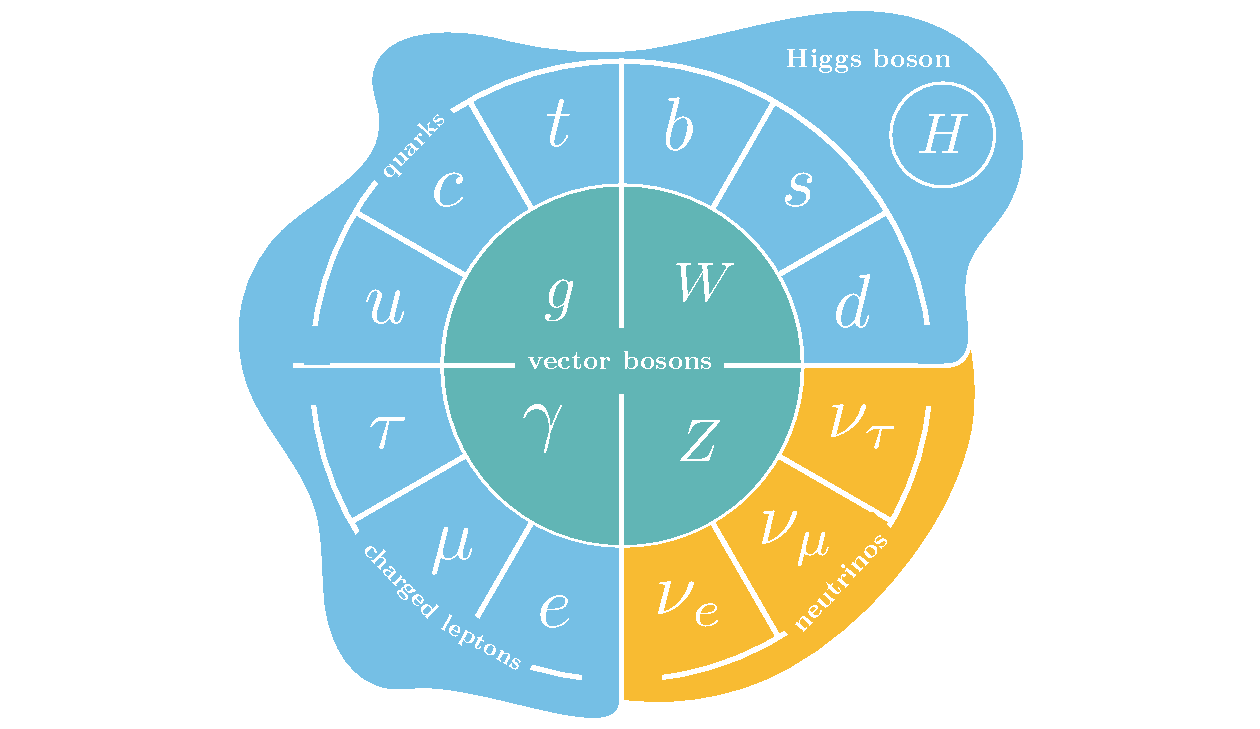
\includegraphics[width=0.85\textwidth]{SM_zoo3.pdf}
 \caption{Artistic rendering of the particles in the Standard Model. \label{fig:SM_diagram}}
\end{figure}
%

Summarizing, the SM particles are illustrated in \reffig{fig:SM_diagram} and the full SM Lagrangian is simply
%
\begin{equation}
 \mathscr{L}_{\rm SM} = \mathscr{L}_{\rm gauge} \,+\, \mathscr{L}_{\rm Higgs}   \,+\, \mathscr{L}_{\rm Yukawa} \,+\, \sum_{\alpha, \Psi}\, \overline{\Psi^\alpha} i \slashed{D} \Psi^\alpha, 
\end{equation}
%
where $\alpha$ is a flavour index and $\Psi \in \{L, Q_L, e_R, u_R, d_R \}$. We saw how a single parameter with massive dimensions in the scalar potential of the SM leads to SSB. This is then ``propagated'' to the rest of the SM through the Higgs kinetic terms and Yukawa couplings. At this point it is possible to appreciate two problems with the SM mass generation mechanism. Firstly, it implies that all Yukawa couplings are just parameters to be inferred from the measured masses of particles. That is, the SM makes no statements and provides no explanations as to why the Yukawas that we observe in nature are what they are. This is known as the flavour puzzle and is equivalent to asking what explains the different observed fermion masses. This problem is aggravated when we consider that neutrinos do have masses and that the leptonic mixing is drastically different from the one in the quark sector. This leads us to the second problem with the SM mass generation. The SM predicts exaclty massless neutrinos in the absence of $\nu_R$ fields. This is perhaps the biggest motivation for studying neutrino physics at present. 

Before moving on to more speculative topics, a few comments are in order. EW SSB seems to be, as far as we know, a real phenomenon. It explains why the symmetries of the SM were so well hidden the first place: true symmetries of Nature seem to not be shared by the vacuum. While the evidence for EW SSB comes mainly from studying fundamental particles, its consequences do not concern only particle physics. EW physics helps us understand the past and future of our own Universe. In the early Universe, at hight temperatures, it is expected that the EW symmetry is restored~\cite{Kirzhnits:1972ut,Dolan:1973qd,Weinberg:1974hy}. If this is the case, the EW phase transition provides a unique test of the Higgs mechanism and points to a completely different Universe from our own, where finite temperature effects and non-perturbative physics play a major role. In addition, we have no reason to expect the vacuum structure of the Universe to be as simple as describe above. After all, the stability of our own vacuum is not even guaranteed within the SM~\cite{Cabibbo:1979ay,Degrassi:2012ry}. Radiative corrections to the Higgs self-coupling $\lambda$ alter the shape of the scalar potential and imply we may live in a local, rather than global, minimum of the potential. For these reasons, studying the Higgs sector, confirming that it generates all fermion masses in the SM and why it seemingly fails to do so in the case of the neutrino are all questions worth pursuing.


%%%%%%%%%%%%%%%%%%%%%%%%%%%%%%%%%%%%%%%%%%%%%%%%%%%%%%%%%%%%%%%%%%%%%%%%%%%%%%%%
%
% BSM!!!!!!
%
%%%%%%%%%%%%%%%%%%%%%%%%%%%%%%%%%%%%%%%%%%%%%%%%%%%%%%%%%%%%%%%%%%%%%%%%%%%%%%%

\section{Evidence for Beyond the Standard Model physics}

The most important building aspects and building blocks of the SM have been laid out above. Now, a different question will concern us: is this theory sufficient to explain fundamental particles and their interactions? In this section we will list what we believe to be the most important hints and evidences that this is not the case. We have already stumbled upon a few problems of the SM, but even before that one must already suspect that the SM is not a final theory. It does not explain gravity. This tells us that the SM should be treated as an effective theory valid up until the Planck mass $M_{\rm Pl} = \left(\hbar c/ 2 G_{\rm Newton}\right)^{1/2} \approx 10^{19}$ GeV, where the effects of gravity are expected to be large~\footnote{This is a naive expectation based on the observation that the Schwarzschild radius $\ell_s = 2 G_{\rm Newton} m/c^2$ and the Compton wavelength $\ell_c = h /mc$ of a particle become comparable at $m \approx M_{\rm Pl}$.}. This very fact already brings us to one of the most debated evidences for beyond the Standard Model (BSM) physics.

\paragraph{The hierarchy problem} The lack of evidence for new physics at the LHC can be argued to be more than just unfortunate. If no new physics is indeed present between the EW and the Planck scale, then the cut-off of the SM, beyond which the effective field theory is no longer valid, is $\Lambda = M_{\rm Pl}$. This implies that unless symmetries are at play, terms of dimensions $d$ are suppressed or are of the order of $\Lambda^{4-d}$. However, in the SM $m_h^2 \ll \Lambda^2$, suggesting a fine-tuning of many orders of magnitude. Quantum corrections to the Higgs mass, $m_h^2 = m^2_{\rm bare} + \delta m_h^2$, are dominated by the top quark and go as $\delta m_h^2 = y_t^2 \Lambda^2 / 8 \pi^2$. This quadratically divergent result implies that to obtain the observed light Higgs mass, whatever new physics that may appear at the scale $\Lambda$ (possibly even below $M_{\rm Pl}$) must cancel the fermion loops to order $m_h^2/ \Lambda^2$. In other words, the matching condition for the renormalization of $m_h^2$ parameter becomes fine-tuned to order $m_h^2/ \Lambda^2$ in the presence of such cut-off. Supersymmetric theories are notorious candidates to solve this problem, but so far we are yet to find any evidence for them. One may argue that indeed there exists a ``desert'' between the EW and the Planck scale, and that some miraculous mechanism is at play in quantum gravity that may solve the fine-tuning problem. In that case, a solution to all following items in this list must be found at that scale, or somewhere outside the realm of particle physics.

\paragraph{The strong-CP problem} The QCD Lagrangian admits the following field-strength contraction term
%
\begin{equation}
 \mathscr{L} \supset \frac{\theta \alpha_s}{8\pi} G_{\mu\nu}^a \tilde{G}_a^{\mu\nu},\quad {\rm where }  \quad \tilde{G}^a_{\mu\nu} = \frac{\epsilon_{\mu\nu\rho\sigma}}{2} {G}^{a\, \rho\sigma}.
\end{equation} 
This can be shown to be a surface term (a total divergence in the action) and can be neglected in perturbative calculations. Nevertheless, this term induces CP violation in the strong sector via non-perturbative effects, leading to a large electric dipole moment for free neutrons~\cite{Crewther:1979pi}, which is orders of magnitude above the experimental upper limits~\cite{Afach:2015sja}. The most popular scenario to explain the smallness of $\theta$ is the Peccei-Quinn symmetry~\cite{Peccei:1977ur}, a global chiral $U(1)$. The breaking of this symmetry leads to the prediction of a pseudo-Nambu-Goldstone boson, the axion.

\paragraph{Matter-antimatter asymmetry} The observed baryon asymmetry of the Universe contradicts the standard Cosmology, which predicts that matter and anti-matter were created in equal amounts in the Big Bang. A good measure of this effect is $\eta_B = (n_B - n_{\overline{B}})/n_\gamma$, where the difference between the number density of baryons and anti-baryons is normalized to the photon number density $n_\gamma$, rendering $\eta_B$ insensitive to the expansion of the Universe. This is measured to be extremely small, $\eta_B = \approx 6 \times 10^{-10}$ with baryons being the dominant component. The SM does not provide enough source of CP violation to explain this phenomenon. Popular scenarios to explain this are EW baryogenesis and leptogenesis. The latter relies on the CP violation from the lepton sector, which is later translated into a baryon asymmetry through non-perturbative spharelon processes that violate total $B+L$ number. This is relevant for neutrino physics, since heavy right-handed neutrinos may realize leptogenesis. 

\paragraph{Dark matter} In the 1930's, Fritz Zwicky measured the velocity dispersion of galaxies in the Coma cluster~\cite{Zwicky:1933gu}, and applied the Virial theorem to show that the matter inferred from its luminosity was insufficient to hold the cluster together. Alongside the pioneering work of Vera Rubin on galaxy rotation curves in the 70's~\cite{Rubin:1970zza}, these observations showed that the gravitational potential in astrophysical scales is much deeper than the one extrapolated from luminous matter. Already at the time, astronomers would refer to the source of this additional gravitational influence as Dark Matter (DM). As astrophysics and cosmology evolved, concrete evidence for DM continued to build up. Now, it is present at a variety of scales, from the precise measurements of the cosmic microwave background (CMB)~\cite{Akrami:2018vks}, the matter distribution in galaxy cluster mergers~\cite{Clowe:2006eq}, and the observed large scale structure of the Universe~\cite{Blumenthal:1984bp}. In fact, from the CMB power spectrum we can infer the DM density today as~\cite{Akrami:2018vks}
\begin{equation}
 \Omega_{\rm DM} h^2 = 0.1200\pm0.0012
\end{equation}
with $\Omega_{\rm DM} = \rho_{\rm DM}/\rho_c$ the energy density of DM in units of the critical density $\rho_c \approx 10^{-26}$ kg/m$^3$, and $h = H_0/(100$ km s$^{-1}$/Mpc$^{-1}) = 0.674\pm0.005$ the scaled Hubble expansion rate. This is roughly five times larger than the density of baryons, understood as all other non-relativistic matter. The latter is also measured through the relative abundances of light elements during Big Bang Nucleosynthesis (BBN)~\cite{Cooke:2013cba}, where DM plays no role, and provides further evidence for the non-baryonic nature of DM.

The nature of DM is not yet understood and many possibilities are under discussion. Modified gravity models explain local astrophysical observations, but struggle to explain all CMB datasets and X-ray observations of mergers of galaxy clusters~\cite{Famaey:2011kh}. Primordial black holes~\cite{Barack:2018yly} have also been put forward as DM candidates and have triggered great interest due to their connection to the detection of gravitational waves. However, the most popular hypothesis at this point remains that DM is made of new particles. This new state better be neutral, to have evaded our detection, and sufficiently long-lived, so that it may linger until today after its production in the early Universe. The fluid of such particles would have to display negligible pressure and viscosity, and to have been created cold so as to help form clumpy structures in the Universe through its gravitational pull. This points us to a particle that is massive, collisionless and, yet, very abundant today. Most notably, DM models have often focused on the possibility of a weakly-interacting massive particle (WIMP). In this paradigm, DM particles, say $\chi$, are produced in the early Universe through its weak interactions with the SM plasma. At later times, approximately at temperatures of the order of the DM mass $m_{\chi}$, DM production stops and annihilation into SM particles dominates. As the Universe cools and expands, the DM gas is diluted and annihilation is no longer effective, \emph{freezing-out} the DM population at around $T \approx m_{\chi}/20$. In particular, the relic density obtained in this mechanism is of the order $\Omega_\chi H_0^2 \approx 0.1 \,{\rm pb}/ \sigma$, where $\sigma$ stands for the thermally averaged cross section of $\chi$ annihilation into SM particles. The fact that $\sigma\approx 1$ pb allows to reproduce the current DM density and is of the order of typical weak cross sections (as in mediated by weak bosons) is known as the WIMP-miracle. WIMP DM is a collisionless and thermal candidate, although DM candidates that are non-thermal, or collisionless, or both exist.

\paragraph{Neutrino masses} One of the most important evidences for BSM physics is the fact that neutrinos have mass. This comes from the plethora of measurements of neutrino oscillations, which we study in the next chapter. Put simply, neutrino oscillation data requires at least 2 non-degenerate massive neutrinos. Although one might argue that this is solved by the mere addition of at least 2 RH singlet states to the SM, this simple extension would require additional theoretical ingredients and experimental confirmation. For instance, such states would be the only SM particle to admit a Majorana mass term of the type $M \,\overline{\nu^c}_R \nu_R$, and unless new symmetries are introduced, there is no reason to expect that $M$ is exactly zero. Therefore, neutrino masses are the first evidence of physics beyond the SM observed in controlled laboratory conditions.


\section{Portals to Beyond the Standard Model}

While we lack a single compelling evidence for the direct detection of a new particle, we can interpret many of the problems outlined above as evidence for new states. The existence of DM and neutrino masses, in particular, suggests (but does not require) that these new states may be a new sector of electromagnetically neutral particles, secluded to their own dark sector. Here, the SM provides little guidance on their masses or symmetries. For this reason, many possibilities to such models exist. We can be guided by experimental anomalous results, by increased elegance in our theories, or by complete agnosticism. In this section we follow take a stronger preference for the latter approach, and set out to discuss the many possibilities through which secluded states may couple to the SM. Much of what we discuss here narrows down the scope of the models we will work with throughout this thesis.

Dark sectors arise in theories where new states, say dark matter particles, are secluded and are not charged under the SM group. These particles may have simple or complicated dynamics in their lair, but their only connection to our SM world is through small \emph{portal couplings}~\cite{Boehm:2003hm,Boehm:2003ha,Alexander:2016aln}. This hypothesis is compelling because it explains why a large fraction of the Universe is invisible to us (in the form of dark states), and why the SM appears so self-contained. The modular and hidden aspect of this point of view is indeed frightening, but this is is not the first time we have encountered it. When Wolfgang Pauli proposed the existence of the neutrino to explain the continuous spectra of electrons from beta decays, he had in fact stumbled upon a key player of a new hidden sector. Initially, in Pauli's own words, this particle was believed to be ``impossible to detect''. It was later clear that this may not be the case if the 4-fermion theory for beta decays by Enrico Fermi was correct. We now know that to be true, where the fact that the neutrino had escaped detection up until that point is explained by the smallness of the fermi coupling constant~\cite{PDG}
\begin{equation}
 \frac{G_F}{\sqrt{2}} = \frac{g^2}{8 M_\textsc{w}^2} = 1.1663787(6) \times 10^{−5}\,\, {\rm GeV}^{−2}.
\end{equation}
In this case, the hidden sector can be thought of as the neutrino, and the weak interactions are our small portal couplings to it. In fact, to study such hidden sector, we had to overcome the smallness of $G_F$ with large exposure experiments at low energies, such as in the detection of neutrinos at just a few meters away from a nuclear reactor by Cowan and Reiness in 1956. Of course, this was not enough to understand the whole picture. As it turns out, $G_F$ is only an effective coupling, and its smallness is simply due to the large masses of the mediators of the weak force. The rest culminates in the construction of the SM. 

With this familiar analogy, we hope that the solution to the problems in the previous sections may display some similar features. Of course, the smallness of portal couplings may not always be due to the high mediator masses. It may arise from a mere accident of the theory, if one believes in such things, from large separation of scales, or from other mechanisms. One realization of small couplings is nicely exemplified by kinetic mixing. In theories with heavy fermions charged both under a new $U(1)$ group and hypercharge, the low energy effects of the new $U(1)$ come in through loop-diagrams like those shown in \reffig{fig:Dark_sectors}. The loop suppression then explains why $\epsilon$, the kinetic mixing parameter, is small $\epsilon \lesssim 10^{-2}$.
%
\begin{figure}[t]
 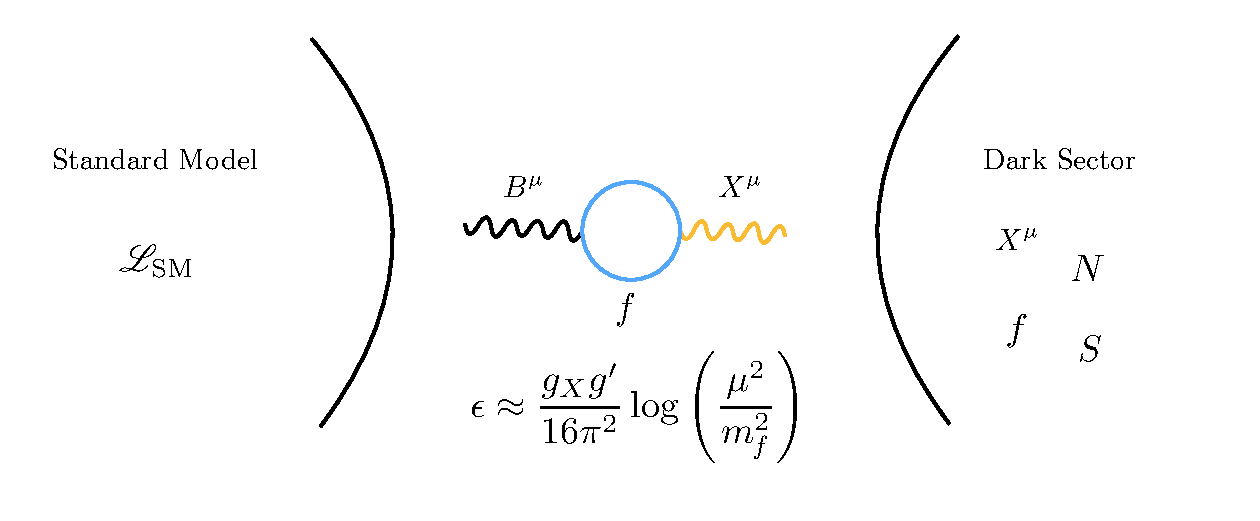
\includegraphics[width=0.95\textwidth]{Dark_sectors.pdf}
 \caption[A possibility for a portal coupling and why it is small.]{A possibility for a portal between the Standard Model and a dark sector. Fermions $f$ charged under both the hypercharge group and a new $U(1)$ group generate kinetic mixing at loop level between $B^\mu$ and the new boson $X^\mu$. In the approximate formula for $\epsilon$, $\mu^2$ stands for the renormalization scale and $g_X$ to the gauge coupling of the new $U(1)$. \label{fig:Dark_sectors}}
\end{figure}
%

To understand the possible links between dark sectors and the SM, we would like to understand all possible ways in which dark and SM particles can interact. One way to tackle this question is to build effective field theories, where one studies all operators which are allowed by the content and symmetries of the SM. The idea is to construct a series of $d>4$ operators in $1/\Lambda^{d-4}$, where $\Lambda$ is the scale of the new physics. This approach thrives on its generality, but can become complicated very quickly with growing $d$. Most importantly, the scale $\Lambda$ is assumed to be large, so that all new degrees of freedom have been integrated out of the theory. This is suitable for extensions involving particles which are very heavy, but the series is no longer well defined for new physics that is light and kinematically accessible at our experiments. In this case, the kinematics of the new particles play a role, forcing us to write down the field content and symmetry group of the new physics. This is the approach we describe in what follows.

We would like our SM extensions to follow specific guiding principles and organize them in a meaningful way. One way to do so is to study all the low dimension neutral operators that the SM has to offer. In contrast to effective field theories, we want renormalizable operators with $d<4$ and that are preferably gauge invariant. As it turns only a few such operators exist, which we usually refer to as \emph{portals}. We dedicate this section to presenting these, as well as the most popular operators that have also been associated with portal couplings, but that are not renormalizable or gauge-invariant.
%
\begin{figure}[t]
 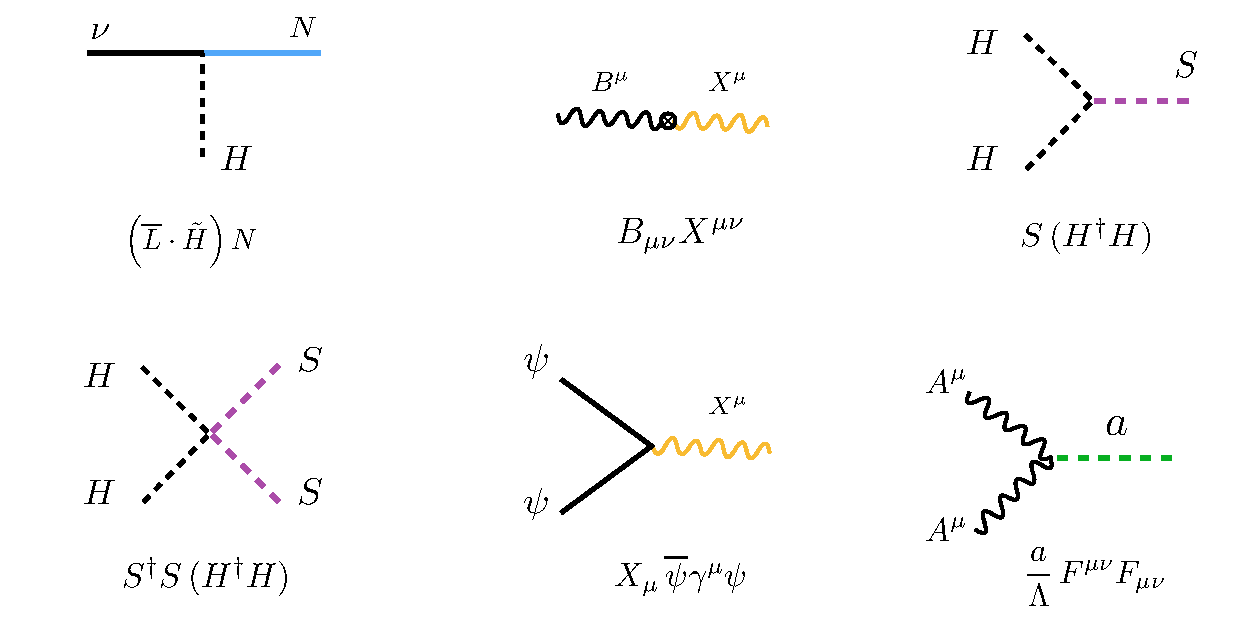
\includegraphics[width=0.95\textwidth]{Dark_portals.pdf}
 \caption[Diagramatic representation of the portal couplings discussed.]{Diagramatic representation of all portal couplings discussed here. From left to right, the top row shows the neutrino, vector and $d=4$ Higgs portal. The bottom row shows the super-renormalizable $d=3$ Higgs portal, the fermionic portal and the non-renormalizable pseudo-scalar portal. \label{fig:all_portals}}
\end{figure}
%

\paragraph{Neutrino portal} Arguably the most motivated portal, this $d=5/2$ operator can be written as
\begin{equation}
\left( \overline{L}^\alpha \cdot \tilde{H}\right).%= \left( \left(\nu^\alpha_L\right)_a \,\, \left(e_L\right)_a \right)
\end{equation}
%
Any fermion field which couples to this operator acquires couplings to SM neutrinos. This typically induces off-diagonal mass terms in the Lagrangian, leading to mixing between the new species and all massive neutrinos in the broken phase of the SM. The new particle is then commonly referred to as \emph{heavy neutral lepton} or right-handed neutrino, though its chirality is a matter of convention. The smallness of this coupling is usually associated to a difference of scales between the EW vev, and the new mass scales of the heavy neutral lepton. We will study such a model in detail in the next chapter.

\paragraph{Vector portal} Any new vector particle $X^\mu$ from an Abelian gauge group may couple to the $d=2$ field strength of the SM hypercharge
\begin{equation}
B_{\mu\nu},
\end{equation}
through its own field strength tensor $X^{\mu\nu}$. The resulting term, $B_{\mu\nu} X^{\mu\nu}$, is a off-diagonal kinetic term for the massive bosons and is sometimes called the \emph{kinetic mixing} operator. This may arise from heavy fermion loops that are integrated out, or through the simultaneous presence of the two Abelian groups across all scales~\footnote{Grand unification clearly forbids such possibility at the highest scales, but this remains, after all, a hypothesis.}. To work in a basis of physical states with diagonal kinetic terms, where the propagators are in their standard form, one usually performs a field redefinition. If much lighter than the EW scale, the new vector particle couples primarily to the EM current, hence the name dark photon. If heavy, it can also couple to the NC and is therefore referred to as a dark $Z$. Models with the term 
%
\begin{equation}
 Z_\mu X^\mu 
\end{equation}
%
also come up in the literature, where it is said that \emph{mass-mixing} between the new vector particle and the SM $Z$ exists. This term is not gauge invariant, but may arise in the broken phase of BSM theories with additional doublet scalars, like in two-Higgs-doublet models (2HDM). In this case, several charged degrees of freedom typically appear and experimental constraints tend to be more severe.

\paragraph{Higgs portal} New scalar particles can couple to the $d=2$ bilinear 
%
\begin{equation}
 H^\dagger H,
\end{equation}
%
the only renormalizable portal with no free Lorentz or spinor indices. In this case there are two possibilities for a scalar to couple to the SM, depending on its charges. We can write  $H^\dagger H \, S^\dagger S$ for a charged, or $H^\dagger H\, S $ for a singlet complex scalar. The latter term is the only super-renormalizable operator connecting the SM fields to new physics which is allowed. Beyond important consequences for EW SSB, these operators typically inherit the Higgs couplings to matter fields, and may be hard to search for due to the smallness of the SM Yukawa couplings. Remarkably, this extension can also have consequences to the hierarchy problem, as the new scalar also contributes to the Higgs self-energy~\cite{Craig:2013xia}.

%
\begin{figure}[t]
 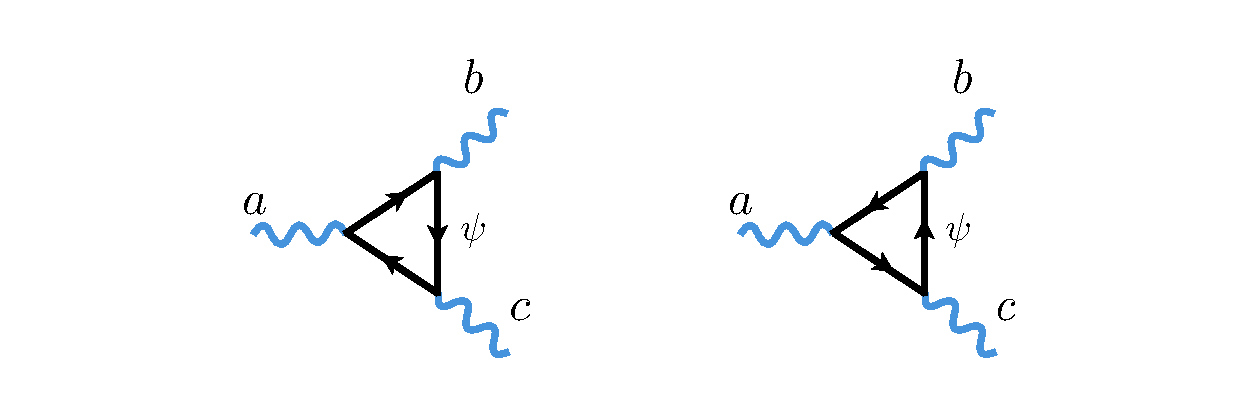
\includegraphics[width=0.8\textwidth]{Triangles.pdf}
 \caption[Anomalous triangle diagrams.]{Anomalous triangle diagrams. The fermion loop is reversed on the right. \label{fig:triangles}}
\end{figure}
%
\paragraph{Fermionic currents}

A whole set of (EM) neutral operators in the SM come from the fermionic currents
\begin{equation}
 J^\mu = \overline{\Psi} \gamma^\mu \Psi,
\end{equation}
where $\Psi \in \{Q_L, L, u_R, d_R, \ell_R\}$. These are not gauge invariant, in general, and will generally require new gauge symmetries to be useful as a portal to the dark sector. The SM currents can be associated with new conserved charges, which in turn may be regarded as a global or promoted to a local gauge symmetry. In the latter case, the new conserved charge is said to be gauged under a local symmetry and additional gauge bosons are introduced, potentially massive. Here, we must also require that it be anomaly-free. This means that the symmetry must be conserved not only classically, but also at loop level. Various types of anomalies exist, but of most interest in gauge extensions of the SM are the chiral gauge anomalies. These can be calculated from the amplitudes of the triangle diagrams shown in \reffig{fig:triangles}, and are proportional to 
%
\begin{equation}
 {\rm Tr}\left[ (T^a T^b + T^b T^a) T^c\right],
\end{equation}
%
where $T^a$ is the group generator corresponding to the gauge boson and in the relevant representation. Here, we take only left-handed particles and anti-particles running in the loop. The simplest case is the one of the $\left[U(1)\right]^3$ chiral anomaly, where it reduces to the requirement that $\sum_\psi Q_\psi^3 = 0$ for all fermions $\psi$ charged under the Abelian group. In the SM, baryon number $B$, lepton number $L$ and the individual lepton number $L_\alpha$ are all accidentally conserved quantities. Non-perturbative effects, however, violate $B$ and $L_\alpha$, and these quantities are no longer conserved~\footnote{Beyond the SM, $L_\alpha$ is already violated at tree-level by the small observed neutrino masses.}. Nevertheless, $B-L$ and the combinations $L_\alpha - L_\beta$ are preserved in these processes and can be taken to be a \emph{global} symmetry of the SM. It is only when gauging these symmetries that one realizes that $B-L$ is, in fact, violated by the chiral triangle diagrams and $L_\alpha - L_\beta$ remains anomaly-free. We explore these leptphilic currents in Abelian extensions of the SM in Chapter 4.

The above exhausts the minimal possibilities for SM portals that lead to renormalizable operators to new physics. Nevertheless, for completeness, we will also comment on a well-motivated non-renormalizable operator that is also frequently discussed in the context of light new physics.


\paragraph{Pseudo-scalar} The Peccei-Quinn solution to the strong CP problem predicts the existence of a new pseudo-scalar $a$, the axion. This is the pseudo-Nambu-Goldstone boson from the breaking of the global $U(1)_{\rm PQ}$ \emph{axial} symmetry at a scale $f_a$. Such particle would then acquire couplings to gauge bosons and SM fermions $\psi$ as in
%
\begin{equation}
 c_1 \, \frac{a}{f_a} G_{\mu\nu}^a \widetilde{G}^{\mu\nu}_{a} + c_2 \, \frac{a}{f_a} W_{\mu\nu}^a \widetilde{W}^{\mu\nu}_{a} + c_3 \, \frac{a}{f_a} B_{\mu\nu} \widetilde{B}^{\mu\nu} +  \sum_\psi c_4^\psi \, \frac{\partial_\mu a}{f_a} \overline{\psi} \gamma^\mu \gamma^5 \psi,
\end{equation}
%
where $c_i$ are model-dependent couplings and are typically linear dependent. Axion particles from models that solve the strong CP problem, commonly referred to as the QCD axions, are not the only possibility. In fact, light pseudo-scalar from the breaking of new symmetries at higher energies provide a well-motivated target for study and go under the name axion-like-particle (ALP). In this case, the relation between the ALP mass and its couplings is less restricted. 
